\begin{figure} [H]
	\vspace{-0.9cm}
\begin{center}
	\scalebox{0.9}{
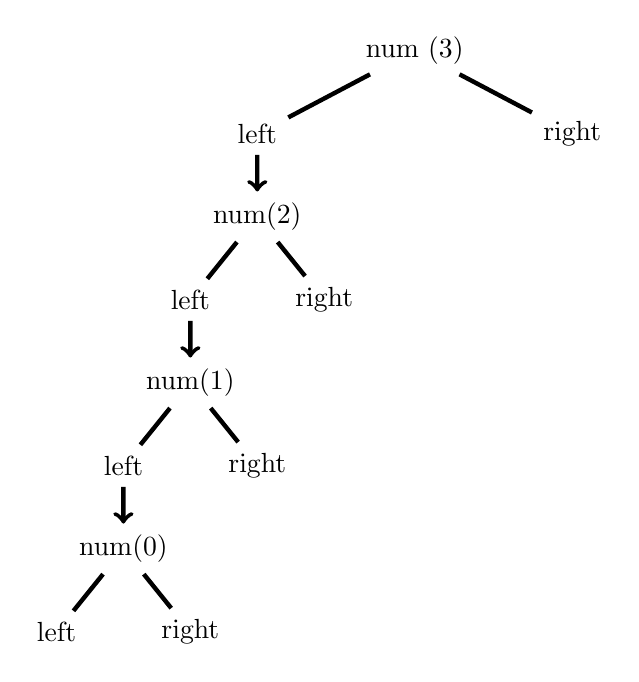
\begin{tikzpicture}
	[
	level distance=30pt,
	level 1/.style={sibling distance=4cm},
	level 2/.style={sibling distance=1.7cm},
	every node/.style = {
	},
	every child/.style = {
		ultra thick
	}
	]
{
\node{num (3)}
	child{node{left}
		child[->]{node{num(2)}
			child[-]{node{left}
				child[->]{node{num(1)}
					child[-]{node{left}
						child[->]{node{num(0)}
							child[-]{node{left}}
							child[-]{node{right}}}}
						child[-]{node{right}}}}
				child[-]{node{right}}
	}}
	child{node{right}};
}
\end{tikzpicture}}
\end{center}
\caption{Representation of a simple number in a computer}
\end{figure}